\clearpage
\begin{proofbox}
\textbf{共同前提：}椭圆与双曲线有相同的两个焦点，
参数满足 $a>c>A>0$（记号见前文），$P$ 为公共点，
$\mathbf u_i=\overrightarrow{F_iP}/PF_i$（$i=1,2$）。
以下按\textbf{最快证明、最低门槛证明、常规坐标法}依次给出，
另附一种完整的切线方程证明。不同方法各有教学价值。

\medskip
\textbf{方法一：最快证明【单位向量的和差，三步】。}

\begin{center}
% u1=(4/5,3/5), u2=(0,1), shown as free vectors based at P.
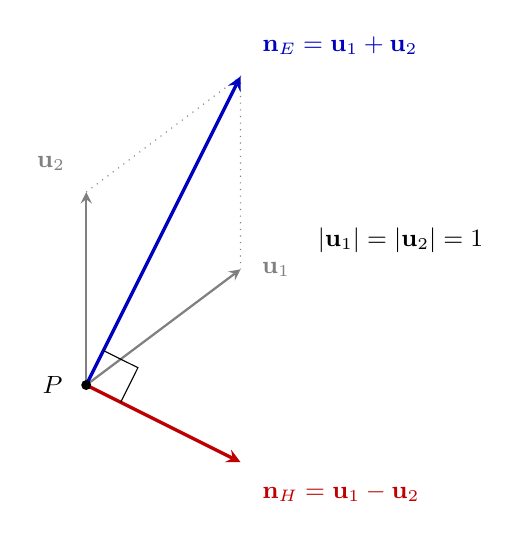
\begin{tikzpicture}[x=2.45cm,y=2.45cm,>=stealth,font=\small]
\draw[gray,dotted] (0,1)--(.8,1.6)--(.8,.6);
\draw[->,gray,thick] (0,0)--(.8,.6) node[right=4pt] {$\mathbf u_1$};
\draw[->,gray,thick] (0,0)--(0,1) node[above left=4pt] {$\mathbf u_2$};
\draw[->,blue!75!black,very thick] (0,0)--(.8,1.6)
 node[above right=4pt] {$\mathbf n_E=\mathbf u_1+\mathbf u_2$};
\draw[->,red!75!black,very thick] (0,0)--(.8,-.4)
 node[below right=4pt] {$\mathbf n_H=\mathbf u_1-\mathbf u_2$};
\draw (.089,.179)--(.268,.09)--(.179,-.089);
\fill (0,0) circle (1.8pt) node[left=5pt] {$P$};
\node[anchor=west] at (1.15,.75) {$|\mathbf u_1|=|\mathbf u_2|=1$};
\end{tikzpicture}


{\small 把单位向量平移到 $P$ 出发，等长使和、差方向垂直。}
\end{center}


\textbf{第1步（识别信号）：}椭圆上两段焦半径之和不变，双曲线同一支上两段焦半径之差不变。
由前文对距离求导得到的关系，垂直于切线的两个向量可分别取为
\[
\mathbf n_E=\mathbf u_1+\mathbf u_2,\qquad
\mathbf n_H=\mathbf u_1-\mathbf u_2.
\]
（左支改变差的符号，不影响法线的方向直线。）

\textbf{第2步（关键计算）：}单位向量长度同为 $1$，因此
\[
\mathbf n_E\cdot\mathbf n_H
=(\mathbf u_1+\mathbf u_2)\cdot(\mathbf u_1-\mathbf u_2)
=1-1=0.
\]
\textbf{第3步（回到目标）：}两个法线方向垂直，
把它们各自转 $90^\circ$ 得到切线，故两切线仍垂直：
\[
\boxed{t_E\perp t_H}.
\]
\textbf{为什么这法最快？}不用解交点、不用繁琐斜率，也无须分左、右支。
\end{proofbox}

\clearpage
\begin{proofbox}
\textbf{方法二：最低门槛证明【焦角的内外角平分线】。}

\begin{center}
% P=(0,0) is a translated copy of (2,3); focal rays (-4,-3),(0,-3).
\begin{tikzpicture}[x=.95cm,y=.95cm,>=stealth,font=\small]
\draw[gray,thick] (0,0)--(-4,-3) (0,0)--(0,-3);
\draw[gray,dotted] (0,0)--(0,1.6);
\draw[orange!80!black,thick,dashed] (-1.7,-3.4)--(.9,1.8);
\draw[teal!85!black,thick,dashed] (-3,1.5)--(2,-1);
\draw[orange!80!black] ({.7*cos(216.86989765)},{.7*sin(216.86989765)})
 arc[start angle=216.86989765,end angle=243.43494882,radius=.7];
\draw[orange!80!black] ({.85*cos(243.43494882)},{.85*sin(243.43494882)})
 arc[start angle=243.43494882,end angle=270,radius=.85];
\draw[teal!85!black] (0,1.05) arc[start angle=90,end angle=153.43494882,radius=1.05];
\draw[teal!85!black] ({1.2*cos(153.43494882)},{1.2*sin(153.43494882)})
 arc[start angle=153.43494882,end angle=216.86989765,radius=1.2];
\draw (.268,-.134)--(.402,.134)--(.134,.268);
\fill (0,0) circle (2pt) node[above right=7pt] {$P$};
\fill (-4,-3) circle (2pt) node[below=5pt] {$F_1$};
\fill (0,-3) circle (2pt) node[below right=5pt] {$F_2$};
\node[orange!80!black,above=5pt] at (.9,1.8) {$t_H$：内角平分线};
\node[teal!85!black,anchor=east] at (-2.5,1.7) {$t_E$：外角平分线};
\node at (-1,-4.1) {内、外角平分线夹角为 $90^\circ$};
\end{tikzpicture}


{\small 焦角的内外角平分线分别是 $t_H,t_E$，不是两条焦半径。}
\end{center}


\textbf{第1步（初中已知）：}连接 $PF_1,PF_2$。设夹角为 $\theta$。
它的内角平分线与外角平分线必互相垂直。

\textbf{第2步（解释切线方向）：}让点沿曲线运动，在 $P$ 处的运动方向就是切线方向。
记两条焦半径的瞬时变化率为 $r_1',r_2'$。
椭圆上 $r_1+r_2$ 不变，故 $r_1'+r_2'=0$；
双曲线上 $|r_1-r_2|$ 不变且所在支固定，
故 $r_1'-r_2'=0$。
因此椭圆切线沿\emph{一段增长、一段缩短}的方向，
恰是焦角外角平分线；双曲线切线沿\emph{两段变化相同}的方向，
恰是焦角内角平分线。

\textbf{第3步（几何结论）：}内、外角平分线垂直，
于是 $t_E\perp t_H$。

\textbf{严谨性补充：}第2步中的“恰是角平分线”并非凭观察猜测。
两条单位焦半径方向为 $\mathbf u_1,\mathbf u_2$，
在它们的\emph{内}角平分线上两个投影相等，
在\emph{外}角平分线上两个投影互为相反数；
这恰好实现 $r_1'-r_2'=0$ 与
$r_1'+r_2'=0$。
\textbf{适用理由：}先用角平分线唤醒初中知识，再用距离的变化率说明切线方向。
\end{proofbox}

\clearpage
\begin{proofbox}
\textbf{方法三：常规坐标法【统一 $a,b,A,B$，联立＋斜率】。}

\begin{center}
% Local exact conics near P=(2,3); tangent slopes -1/2 and 2.
\begin{tikzpicture}[x=.95cm,y=.95cm,font=\small]
\draw[blue!75!black,thick,domain=10:105,samples=90,variable=\t]
 plot ({4*cos(\t)},{sqrt(12)*sin(\t)});
\draw[red!75!black,thick,domain=.3:4.9,samples=90,variable=\t]
 plot ({sqrt(1+\t*\t/3)},\t);
\draw[teal!85!black,thick,dashed] (-.5,4.25)--(4.8,1.6);
\draw[orange!80!black,thick,dashed] (.6,.2)--(3,5);
\node[teal!85!black,anchor=west] at (4.6,2.15) {$k_E=-\tfrac12$};
\node[orange!80!black,above right=4pt] at (3,5) {$k_H=2$};
\draw (2.358,2.821)--(2.537,3.179)--(2.179,3.358);
\fill (2,3) circle (2.4pt) node[above left=8pt] {$P$};
\node at (1.5,-.55) {$k_Ek_H=-1$};
\end{tikzpicture}


{\small 图取 $P=(2,3)$；一般交点的斜率积也为 $-1$。}
\end{center}


设焦点 $F_1=(-c,0),F_2=(c,0)$（$c>0$），分别写为
\[
 E:\ \frac{x^2}{a^2}+\frac{y^2}{b^2}=1,\qquad
 H:\ \frac{x^2}{A^2}-\frac{y^2}{B^2}=1.
\]
其中 $a>b>0$，$A,B>0$，\textbf{共焦先给出}
\[
\boxed{a^2-b^2=A^2+B^2=c^2},\qquad
\boxed{a^2-A^2=b^2+B^2}.
\]
\textbf{第1步（为何联立）：}交点 $P=(x_0,y_0)$ 同时满足两个方程。
令 $U=x_0^2,V=y_0^2$，变为线性方程组
\[
\begin{cases}
 U/a^2+V/b^2=1,\\
 U/A^2-V/B^2=1.
\end{cases}
\]
由第一式得 $V=b^2(1-U/a^2)$，第二式得
$V=B^2(U/A^2-1)$，令两式相等：
\[
 b^2+B^2=U\left(\frac{b^2}{a^2}+\frac{B^2}{A^2}\right).
\]
\textbf{为什么此时用共焦条件？}右侧系数的分子可因式分解：
\[
 A^2b^2+a^2B^2
 =A^2(b^2+B^2)+B^2(a^2-A^2)
 =c^2(b^2+B^2).
\]
于是 $b^2+B^2>0$ 可消去，得到
\[
\boxed{x_0^2=\frac{a^2A^2}{c^2}},\qquad
\boxed{y_0^2=\frac{b^2B^2}{c^2}}.
\]
\textbf{几何信息：}两个平方严格大于 $0$，因此恰有
$P=(\pm aA/c,\pm bB/c)$ 四个不同交点；两正负号独立。

\end{proofbox}
\clearpage
\begin{proofbox}
\textbf{方法三（续）：从交点坐标走向切线方向。}

\textbf{第2步（隐函数求导）：}椭圆、双曲线的切线斜率为
\[
\boxed{k_E=-\frac{b^2x_0}{a^2y_0}},\qquad
\boxed{k_H=\frac{B^2x_0}{A^2y_0}}.
\]
这里 $x_0y_0\ne0$，所以两条斜率均存在。

\textbf{第3步（代入交点关系，立即消去）：}
\[
\begin{aligned}
 k_Ek_H
 &=-\frac{b^2B^2x_0^2}{a^2A^2y_0^2}\\
 &=-\frac{b^2B^2}{a^2A^2}\cdot
 \frac{a^2A^2}{b^2B^2}=\boxed{-1}.
\end{aligned}
\]
故两条切线垂直。
\textbf{条件分工：}共焦控制参数，公共点控制坐标，求导控制切线方向。
\textbf{为什么需要公共点条件？}仅凭参数平方恒等式不能代入任意点的
$x^2/y^2$；恰恰是“同一点同时在两曲线上”给出了上述比值。
\end{proofbox}

\clearpage
\begin{proofbox}
\textbf{方法四：补充证明【切线方程＋法向量点积】。}

\begin{center}
% N_E=(1/8,1/4); N_H=(2,-1); arrows are positive scalar multiples.
\begin{tikzpicture}[x=1cm,y=1cm,>=stealth,font=\small]
\draw[teal!85!black,dashed,thick] (-1,4.5)--(5,1.5);
\draw[orange!80!black,dashed,thick] (.7,.4)--(3.1,5.2);
\draw[->,blue!75!black,very thick] (2,3)--(2.7,4.4);
\draw[->,red!75!black,very thick] (2,3)--(3.4,2.3);
\node[blue!75!black,anchor=west] at (3.05,4.55) {$\parallel\mathbf N_E$};
\node[red!75!black,anchor=west] at (3.7,2.65) {$\parallel\mathbf N_H$};
\node[teal!85!black,anchor=west] at (4.6,1.35) {$t_E$};
\node[orange!80!black,above] at (3.1,5.25) {$t_H$};
\draw (2.134,3.268)--(2.402,3.134)--(2.268,2.866);
\fill (2,3) circle (2.2pt) node[left=8pt] {$P$};
\node at (1.5,-.2) {实箭头：法向量；虚线：切线};
\end{tikzpicture}


{\small 箭头按正比例缩放，两法向量分别垂直于各自切线。}
\end{center}


沿用方法三中 $P=(x_0,y_0)$ 和共焦参数。
两条切线方程为
\[
 t_E:\ \frac{x_0x}{a^2}+\frac{y_0y}{b^2}=1,\qquad
 t_H:\ \frac{x_0x}{A^2}-\frac{y_0y}{B^2}=1.
\]
对应法向量可取
\[
\mathbf N_E=\left(\frac{x_0}{a^2},\frac{y_0}{b^2}\right),\qquad
\mathbf N_H=\left(\frac{x_0}{A^2},-\frac{y_0}{B^2}\right).
\]
用交点坐标平方式 $x_0^2=a^2A^2/c^2$、
$y_0^2=b^2B^2/c^2$，直接求得
\[
\begin{aligned}
\mathbf N_E\cdot\mathbf N_H
 &=\frac{x_0^2}{a^2A^2}-\frac{y_0^2}{b^2B^2}\\
 &=\frac1{c^2}-\frac1{c^2}=\boxed{0}.
\end{aligned}
\]
法向量垂直，故切线也垂直。
\textbf{为什么保留此法：}写切线方程时无需先求斜率；
它也能迁移到斜率不存在的其他曲线问题。
\end{proofbox}
